\chapter{Implications for the Standard Model and Cosmology}\label{chapter:SM_Cosmology}

% - Pati-Salam unification: all fermions represented by four copies of KD fermions.
% - Kinetic terms, Yukawa coupling, Majorana mass term.
% - SU(4), subgroup SU(3), and V=U(2)xU(2), if we only focus on one sheet, U(2)=SU(2)xU(1). In total SU(3)xSU(2)xU(1) --> show the gauged equation, with gauged fields acting from the right. 
% - Remaining problems: why weak force only act on LH particles? Why three generations? Might get answer from twistor theory.
% - CPT-symmetric universe, BH mirror (also discuss How Gerard 't Hooft's BH theory describe thermolize and information paradox)would describe how to 

\chapterabstract{In this chapter, we explore the implications of Kähler-Dirac (KD) fermions for both the Standard Model (SM) of particle physics and cosmology. Within the SM framework, the 16 Weyl fermions comprising a single generation are elegantly represented by four copies of a KD-Majorana field. The complete SM gauge group, $SU(3)\times SU(2)\times U(1)$, naturally emerges from the internal symmetry of the KD field combined with transformations among three of these four copies. Furthermore, the fermionic kinetic terms, Yukawa couplings, and right-handed neutrino Majorana mass terms are systematically constructed within this unified KD formulation. Turning to cosmology, the inherent two-sheeted topological structure of the KD field naturally accommodates the $CPT$-symmetric universe model. Crucially, the KD-Majorana condition provides a rigorous theoretical explanation for why the universe and anti-universe must remain perfectly $CPT$-symmetric, even at the quantum scale. Finally, this constraint justifies the fundamental assumption underlying the black hole (BH) mirror model, which states that a black hole's event horizon acts as an additional $CPT$-symmetric mirror bridging the two spacetime sheets, where the infalling particles would annihilate with their anti-particles coming from the anti-universe.}

\section{Relation to the Standard Model}\label{sec:SM}

% Editor's note: Elevated the conversational phrasing to a more formal academic tone.
On one hand, a single Standard Model (SM) generation (including a right-handed neutrino) is fully described by 16 independent Weyl spinor fields. On the other hand, a single Kähler-Dirac (KD) field satisfying the KD-Majorana condition inherently contains two Dirac spinors (the other two are their anti-particles living in the other sheet), which equates to four Weyl spinors. Consequently, exactly four KD-Majorana fields are required to represent a full fermion generation. To allocate the leptons and quarks into these four copies ($\Psi'_{\!A=0,\ldots,3}$), we follow the idea from Catterall \cite{Catterall:2023nww} by adopting 4 KD fields into the foundational framework of the Pati-Salam unification scheme \cite{Pati:1974yy}.

The first copy represents the lepton sector: 
\begin{equation}\label{eq:Psi_leptons}
  \Psi'_{0}=\chi_{0}+\chi_{0}^{c},\quad \text{where } \chi_{0}=\left(\begin{array}{cccc}
    \nu_{L} & e_{L} & 0 & 0 \\
    \nu_{R} & e_{R} & 0 & 0 \end{array}\right),
\end{equation} 
where all non-zero entries in this matrix are 2-component Weyl spinors. The subsequent three copies ($\Psi'_{i=1,2,3}$) represent the three colors of quarks:
 \begin{equation}\label{eq:Psi_quarks}
   \Psi'_{i}=\chi_{i}+\chi_{i}^{c},\quad \text{where }\chi_{i}=\left(\begin{array}{cccc}
    u_{L}^{i} & d_{L}^{i} & 0 & 0 \\
    u_{R}^{i} & d_{R}^{i} & 0 & 0 \end{array}\right).
 \end{equation}

We now demonstrate how all fundamental fermion interactions in the Standard Model can be seamlessly rewritten within this KD framework.

\subsection{The KD Kinetic Term}

The SM fermion kinetic terms naturally unify into the following compact trace:
\begin{equation}
    \mathcal{L}_{\text{KD}} = \text{Tr}[\bar{\Psi}_{\!A}(i\partial\!\!\!\!\;\!/\,)\Psi_{\!A}]=
    \text{Tr}[\Lambda \Psi_{\!A}'^{\dagger}\gamma^{0}(i\partial\!\!\!\!\;\!/\,)\Psi_{\!A}'],
\end{equation}
where the copies index $A=0,\ldots,3$ is implicitly summed over. In addition to the $Spin(3,1)_{{\rm Lorentz}}\times U(2,2)_{{\rm internal}}$ symmetry described in the previous chapter, this specific action also possesses a global internal $SU(4)$ symmetry that permutes the four copies of $\Psi'$ (acting on $A=0,\ldots,3$). 

To recover the SM interactions, we gauge an $SU(3)$ subgroup of this overarching $SU(4)$ symmetry, allowing only the three colors of quarks transform. Furthermore, as demonstrated in the previous chapter \cref{subsec:KD-Majorana_constrain_internal_symm}, the internal symmetry is rigorously restricted to $V=U(2)\times U(2)$, where the two $U(2) \cong SU(2)\times U(1)$ factors act as exact charge conjugates of one another. Because $V$ is block-diagonal, $V=\begin{pmatrix}A &0\\ 0&B\end{pmatrix}$, it acts independently on the particles and antiparticles residing on the forward and backward sheets, respectively. By restricting our focus strictly to a single sheet, we naturally recover the full SM gauge group, $SU(3)\times SU(2)\times U(1)$. Replacing the standard derivative $\partial\!\!\!\!\;\!/$ with the appropriate gauge covariant derivative yields the complete SM fermion kinetic Lagrangian (including all requisite gauge interactions). 

We explicitly write this covariant derivative as:
\begin{equation}
\begin{aligned}
    D_\mu\Psi_L'^i&=(\partial_\mu+ig_3 G_{\mu,j}^i)\Psi'^j_L+ig_2\Psi'^i_L \mathcal W_\mu+ig_1\frac{2}{3}\Psi'^i_L \mathcal B_\mu,\\
    \mathcal W_\mu&=\begin{pmatrix}W_\mu &0\\ 0 & W_\mu^c\end{pmatrix}, \text{ where } W_\mu^c=\sigma^2W_\mu^*\sigma^2, \\ \mathcal{B}_\mu&=\begin{pmatrix}B_\mu &0\\ 0 & B_\mu^c\end{pmatrix}, \text{ where } B_\mu^c=B_\mu^*.
\end{aligned}
\end{equation}
Similarly, the covariant derivative for the right-handed quarks $\Psi_R^i$ is obtained by omitting the weak term $\mathcal W_\mu$. For the leptons, the derivative for $\Psi_L^0$ is constructed by omitting the strong term $G_\mu$, and finally, the derivative for $\Psi_R^0$ is constructed by omitting both $\mathcal W_\mu$ and $G_\mu$.

\vspace{0.25cm}
% Editor's note: Removed the trailing colon after the section command to prevent formatting errors.
\subsection{Yukawa Couplings}

Having outlined the kinetic structure, we now translate the Yukawa couplings into the KD formulation. 
Recall that the standard Yukawa Lagrangian ${\cal L}_{Y}$ (including interactions with a right-handed neutrino) takes the conventional form:
\begin{equation}\label{eq:Yukawa_standard}
     \tilde{h}^{T}\!\bar{q}_L^{\,i}u_R^j y_u^{ij} + 
     h^{T}\!\bar{q}_L^{\,i}d_R^j y_d^{ij} + \tilde{h}^{T\;\!}\!\bar{\ell}_L^{\,i}\nu_R^j y_\nu^{ij} + h^{T\;\!}\!\bar{\ell}_L^{\,i} e_R^j y_e^{ij} + \text{h.c.}
\end{equation}
Here, $h$ is the SM Higgs doublet, and $\tilde{h}\equiv i\sigma^{2}h^{\ast}$. The matrices $y_{u}^{ij}$, $y_{d}^{ij}$, $y_{\nu}^{ij}$, and $y_{e}^{ij}$ represent complex $3\times 3$ Yukawa matrices, where $i,j\in \{1,2,3\}$ denote the generation indices. The fields $q_{L}=(u_{L},d_{L})$ and $\ell_{L}=(\nu_{L},e_{L})$ are the left-handed quark and lepton doublets (written as standard $2\times2$ matrices). Note that in this specific section, we temporarily revert to the conventional (non-KD) bar notation for spinors (e.g., $\bar{q}_{L}=q_{L}^{\dagger}\gamma^{0}$, without the extra $\gamma^{0}$ acting from the left).

These disparate Yukawa couplings can be elegantly compressed within the KD formalism as follows:
\begin{equation}\label{eq:Yukawa_KD}
    \mathcal{L}_{Y}=
    \text{Tr}[\mathcal{H}^{\top}\widehat{\Psi}_{A,L}'^{i}\Psi_{A,R}'^j \mathcal{Y}_A^{ij}] + \text{h.c.}  
\end{equation}
,where $\widehat{\Psi}' \equiv \Lambda \Psi'^\dagger \gamma^0$ to distinguish it from the bar notation for standard Dirac spinors. The generalized KD Higgs field ${\cal H}$ and the unified Yukawa coupling matrices ${\cal Y}^{ij}_{A}$ are explicitly defined below.

Let us demonstrate how this unified expression explicitly recovers the standard couplings for the lepton sector ($A=0$) \cref{eq:Yukawa_standard}. The fundamental building blocks are the $4 \times 4$ matrices for the lepton field $\Psi_0$, the unified Higgs field $\mathcal{H}$, and the Yukawa couplings $\mathcal{Y}_0$:
\begin{gather}
    \Psi_{0,L}'=\begin{pmatrix} \ell_L & 0 \\ 0 & \ell_L^c \end{pmatrix}, \quad
    \Psi_{0,R}'=\begin{pmatrix} 0 & \ell_R^c \\ \ell_R & 0 \end{pmatrix}\\
    \mathcal{H} = \begin{pmatrix} H & 0 \\ 0 & H^{c} \end{pmatrix}, \quad \text{where } H=H^c=(\tilde h, h) \\
    \!\!\mathcal{Y}_0^{ij} = \begin{pmatrix}
        Y_0^{ij} & 0 \\ 0 & Y_0^{c,ij}
    \end{pmatrix}, \quad
    \begin{aligned}
        Y_0^{ij} &= \text{diag}(y_\nu^{ij}, y_e^{ij}), \\
        Y_0^{c,ij} &= \text{diag}(y_e^{ij*}, y_\nu^{ij*}),
    \end{aligned}
\end{gather}
with the conjugate relationships defined as $H^c=\sigma^2H^*\sigma^2$ and $Y_0^{c,ij}=\sigma^2Y_0^{ij,*}\sigma^2$.

Applying these definitions to expand \cref{eq:Yukawa_KD} yields:
\vspace{-0.1cm}
\begin{equation}\label{eq:yukawa_expand}
\begin{aligned}
    &\text{Tr}[\mathcal{H}^{\top}\widehat{\Psi}_{0,L}'^{i}\Psi_{0,R}'^j \mathcal{Y}_0^{ij}] \nonumber \\
    &=\text{Tr}[H^{\top}\bar{\ell}_{L}^{\,i}\ell_{R}^{\,j} Y_0^{ij}] - \text{Tr}[H^{\,c,\top}\bar{\ell}_{L}^{\,c,i}\ell_{R}^{\,c,j} Y_0^{c,ij}].
\end{aligned}
\end{equation}
The first term precisely dictates the Yukawa couplings acting on the forward sheet, while the second term captures the analogous couplings on the backward sheet.

To verify this, we further expand the $2\times 2$ components of the first term, $\text{Tr}[H^{\top}\bar{\ell}_{L}^{\,i}\ell_{R}^jY_0^{ij}]$: 
\begin{equation}
\begin{aligned}
    \text{Tr}[H^\top\bar{\ell}_{L}^{\,i}\ell_{R}^jY_0^{ij}]
    =\tilde{h}^\top\bar{\ell}_{L}^{\,i} \nu_R^j y_\nu^{ij}+h^\top \bar{\ell}_{L}^{\,i}e_R^j y_e^{ij}.
\end{aligned}
\end{equation}
This beautifully reproduces the two required standard Yukawa coupling terms for the lepton sector. Following identical mathematical logic, expanding the second term in \cref{eq:yukawa_expand} yields the strictly required corresponding couplings for antiparticles residing on the ``other" $PT$-reversed sheet. 

Applying this exact methodology to the quark sector ($\Psi_i$) reliably generates all remaining Yukawa couplings of the Standard Model. Thus, (\ref{eq:Yukawa_KD}) successfully and comprehensively unifies all Yukawa interactions.

% Editor's note: Improved grammatical structure and clarity of the PT-reversal proofs.
Finally, we must verify whether this Yukawa Lagrangian remains positive-definite after a full $PT$ reversal, mirroring the calculation performed in \cref{sec:Two-sheeted_spacetime}.
Recall that $4\times 4$ spinors $X$ transform under $PT$ reversal as $(PT)X(PT)^{-1}$, where the operator is defined as $(PT)=\eta \gamma^0\gamma^1\gamma^3K=\eta\begin{pmatrix}0&\sigma^2\\ \sigma^2&0\end{pmatrix}K$. This transformation yielded $ \tilde \Psi'(x)=\begin{pmatrix}\ell_L(x)&-\ell_R^c(\tilde x)\\ \ell_R(x) & \ell_L^c(\tilde x)\end{pmatrix}$. Applying this same transformation to the unified Higgs field $\mathcal{H}$ gives: 
\begin{equation}
\begin{aligned}
    (PT)\mathcal{H}(PT)^{-1}&=\eta\begin{pmatrix}0&\sigma^2\\ \sigma^2&0\end{pmatrix}K \begin{pmatrix} H & 0 \\ 0 & H^{c} \end{pmatrix}K^{-1}\begin{pmatrix}0&\sigma^2\\ \sigma^2&0\end{pmatrix}\eta^{-1}\\
    &=\begin{pmatrix}0&\sigma^2\\ \sigma^2&0\end{pmatrix}\begin{pmatrix} H^* & 0 \\ 0 & (H^{c})^* \end{pmatrix}\begin{pmatrix}0&\sigma^2\\ \sigma^2&0\end{pmatrix}\\
    &=\begin{pmatrix}\sigma^2(H^{c})^*\sigma^2  & 0 \\ 0 & \sigma^2H^*\sigma^2 \end{pmatrix}=\begin{pmatrix} H & 0 \\ 0 & H^{c} \end{pmatrix}=\mathcal{H}.
\end{aligned}
\end{equation}

Similarly, it is straightforward to show that $(PT)\mathcal{Y}_A(PT)^{-1}=\mathcal{Y}_A$. Therefore, both $\mathcal{H}$ and $\mathcal{Y}_A$ are mathematically invariant under $PT$ reversal.

Substituting these transformed components back into the Yukawa Lagrangian yields: 
\begin{equation}
\begin{aligned}
    &\tilde{\mathcal{L}}_{Y}=
    \text{Tr}[\tilde {\mathcal{H}}^{T}\Lambda(\tilde\Psi_{L}'^{i})^\dagger\gamma^0\tilde\Psi_{R}'^j \tilde{\mathcal{Y}}^{ij}] + \text{h.c.} \\
    &=\text{Tr}\left[\begin{pmatrix} H & 0 \\ 0 & H^{c} \end{pmatrix}\begin{pmatrix} \mathbbm{1} & 0 \\ 0 & -\mathbbm{1} \end{pmatrix}\begin{pmatrix}\ell_L(x)^\dagger&0\\ 0 & (\ell_L^c(\tilde x))^\dagger\end{pmatrix}\begin{pmatrix} 0 & \mathbbm{1} \\ \mathbbm{1}& 0 \end{pmatrix}\begin{pmatrix}0&-\ell_R^c(\tilde x)\\ \ell_R(x) &0 \end{pmatrix} \begin{pmatrix} Y & 0 \\ 0 & Y^{c} \end{pmatrix}\right] + \text{h.c.}\\
    &=\text{Tr}[H\ell_L^\dagger\ell_RY]+\text{Tr}[H^c(\ell_L^c)^\dagger\ell_R^cY^c]+ \text{h.c.}
\end{aligned}
\end{equation}
This confirms that the unified Yukawa Lagrangian is robustly positive-definite across both sheets.

\vspace{0.25cm}
% Editor's note: Removed the trailing colon after the section command to prevent formatting errors.
\subsection{The Right-Handed Neutrino Majorana Mass Term}

The final fermion interaction term in the Standard Model (when right-handed neutrinos are included) is the RH neutrino Majorana mass term ${\cal L}_{M}$, which is conventionally written as:
\begin{equation}
  {\cal L}_{M}=\bar{\nu}_R^{\,c,i}\nu_{R}^{\,j}m^{ij}+\text{h.c.},
\end{equation}
where $m^{ij}$ is a symmetric $3\times3$ mass matrix that, without any loss of theoretical generality, can be rendered entirely real via appropriate field redefinitions. In the KD formalism, this term transforms into the trace:
\vspace{-0.1cm}
\begin{equation}
  {\cal L}_{M}={\rm Tr}[\widehat{\Psi}_{A,R}'^{i}\Psi_{A,R}'^{j}\mathcal{M}_{A}^{ij}],
\end{equation}
where KD Majorana mass matrix ${\cal M}_{A}^{ij}$ is:
\begin{equation}
  {\cal M}_{A}^{ij}= \begin{pmatrix}0 & M^{c,ij} \\
  M^{ij} & 0 \end{pmatrix}
  \delta_{A}^{0},\quad
  \text{where } M^{ij}=\begin{pmatrix} 0 & 0 \\
  m^{ij} & 0 \end{pmatrix}.
\end{equation}

Note that, exactly as observed in the free KD theory discussed above, the KD-Majorana condition fundamentally implies that across all Standard Model fermion terms (kinetic, Yukawa, and Majorana mass), the action evaluated on the forward sheet is precisely equal to the action on the backward sheet (meaning they would naively cancel out entirely if interpreted from a single-sheeted perspective). 

Finally, we verify that this mass term also becomes positive-definite under $PT$ reversal:
\begin{equation}
\begin{aligned}
    (PT){\cal M}(PT)^{-1}&=\eta\begin{pmatrix}0&\sigma^2\\ \sigma^2&0\end{pmatrix}K \begin{pmatrix} 0 & M^c \\ M & 0 \end{pmatrix}K^{-1}\begin{pmatrix}0&\sigma^2\\ \sigma^2&0\end{pmatrix}\eta^{-1}\\
    &=\begin{pmatrix}0&\sigma^2\\ \sigma^2&0\end{pmatrix} \begin{pmatrix} 0 & (M^c)^* \\ M^* & 0 \end{pmatrix}\begin{pmatrix}0&\sigma^2\\ \sigma^2&0\end{pmatrix}=\begin{pmatrix} 0 & \sigma^2M^*\sigma^2 \\ \sigma^2(M^c)^*\sigma^2 & 0 \end{pmatrix}\\
    &=\begin{pmatrix} 0 & -M^c \\ -M & 0 \end{pmatrix}=-{\cal M}.
\end{aligned}
\end{equation}
Here, we utilized the property that since $M=\begin{pmatrix}0&0\\m&0\end{pmatrix}$, its conjugate is $ M^c=-\sigma^2M^*\sigma^2$.

Following the established procedure, we invert the sign solely for the matrix components residing on the backward sheet: $\tilde{\cal M}=\begin{pmatrix} 0 & -M^c(\tilde x) \\ M(x) & 0 \end{pmatrix}$.
Substituting this back into the Lagrangian yields: 
\begin{equation}
\begin{aligned}
    {\cal L}_{M}&={\rm Tr}\left[\Lambda({\tilde\Psi}_{R}'^{i})^\dagger\gamma^0\tilde\Psi_{R}'^{j}\tilde{\mathcal{M}}^{ij}\right] \\
    &={\rm Tr}\left[\begin{pmatrix} \mathbbm{1} & 0 \\ 0 & -\mathbbm{1} \end{pmatrix}\begin{pmatrix}0&\ell_R^\dagger\\ -(\ell_R^c(\tilde x))^\dagger &0 \end{pmatrix} \begin{pmatrix} 0 & \mathbbm{1} \\ \mathbbm{1}& 0 \end{pmatrix}\begin{pmatrix}0&-\ell_R^c(\tilde x)\\ \ell_R(x) &0 \end{pmatrix} \begin{pmatrix} 0 & M^c \\ M & 0 \end{pmatrix}\right] \\
    &=-\big(\rm Tr[\ell_R^\dagger\ell_R^c M]+\rm Tr[(\ell_R^c)^\dagger\ell_RM^c]\big).
\end{aligned}
\end{equation}

All terms enclosed within the bracket represent strictly positive-definite quantities. Although there is an overall global minus sign leading the Lagrangian, this poses no physical pathology, as the overall sign of the action can be freely redefined without altering the resulting equations of motion.

\vspace{0.25cm}
\section{Cosmological Implications}\label{sec:KD_cosmology}

\subsection{Connections to the $CPT$-Symmetric Universe }
% Editor's note: Enhanced transitions and corrected grammatical errors (e.g., "thermolize" -> "thermalize", "how BH growth" -> "how black holes grow").
It is deeply natural to wonder about the broader physical implications of this two-sheeted spacetime architecture, particularly one governed by a strict KD-Majorana symmetry that mathematically ties the two sheets together.

Specifically, it is highly intriguing to speculate on its implications for cosmology. One can theoretically conceptualize the forward and backward sheets as representing the epochs ``after" and ``before" the Big Bang, inherently joined at the initial singularity itself \cite{Boyle:2021jej}. This topological configuration aligns strikingly well with the $CPT$-Symmetric Universe model discussed in introduction \cref{chapter:introduction}, wherein the Big Bang functions as a temporal mirror joining a universe/anti-universe pair via exact $CPT$ symmetry. However, the fundamental mechanism driving these reflecting boundary conditions remained somewhat phenomenological. Why must the Big Bang act as a rigorous $CPT$ mirror? The KD-Majorana condition proposed here—which is strictly necessary to formulate a physically consistent theory of KD fermions—appears to provide a highly elegant, fundamental quantum explanation. 

\subsection{Application to the Black Hole Mirror Model}

Relatedly, the ``black mirror" hypothesis was recently proposed as a radical alternative to the standard physics of black holes. In this novel framework, the standard black hole interior does not exist; instead, the event horizon serves as a another $CPT$-symmetric mirror bridging our exterior spacetime directly to the ``other" exterior in anti-universe \cite{tzanavaris2025blackmirrorscptsymmetricalternatives}. Under this topology, every infalling particle from our universe would annihilate perfectly with its corresponding infalling antiparticle arriving from the anti-universe exactly at the horizon (see \cref{fig:annihilate_BHmirror}). However, there is the hidden assumption that the universe and anti-universe are totally CPT-symmetric, even in quantum scale. The KD-Majorana condition naturally provide the theoretical explanation.

\begin{figure}[htbp]
     \centering
     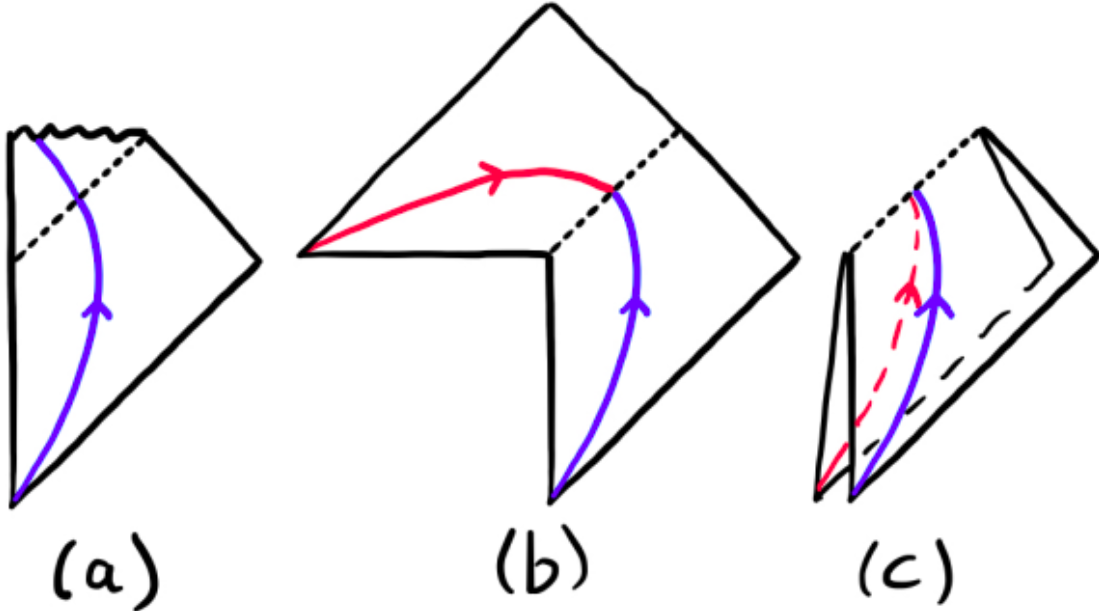
\includegraphics[width=0.65\textwidth]{parts/part2/figures/annihilate_BHmirror.png}
     \caption{In the black hole mirror model, the event horizon acts as a $CPT$-symmetric mirror connecting the exterior of our universe to the exterior of anti-universe. Infalling matter from our universe annihilates with infalling antimatter from the anti-universe at the horizon. The KD-Majorana condition provides a fundamental explanation for why the universe and anti-universe must remain perfectly $CPT$-symmetric, even at quantum scales.}
     \label{fig:annihilate_BHmirror}
\end{figure}

One might ask what physically transpires immediately following this horizon annihilation. There are two primary hypothetical scenarios: upon annihilation, the infalling matter is either (1) converted into photons permanently bound to travel along the event horizon, and/or (2) converted into Hawking radiation that is immediately emitted back outward into both the universe and the anti-universe. Both scenarios, however, face unresolved theoretical challenges.

Scenario (1) is conceptually appealing because it links directly to Hawking's original macroscopic description, where all in-falling information is holographically encoded on the event horizon, thereby dictating the Bekenstein-Hawking entropy. However, the critical challenge facing this scenario is that the presence of high-energy photons on the event horizon results in a non-zero energy-momentum tensor exactly at the boundary. This boundary is therefore no longer a true vacuum, which fundamentally violates the foundational mathematical assumptions of the purely vacuum Schwarzschild metric. Obtaining a mathematically consistent metric solution that accommodates this boundary energy likely requires complex numerical gravity treatments.

Scenario (2) postulates that the photons produced by the annihilation immediately escape as observable Hawking radiation. This scenario is highly attractive because it trivially resolves the black hole information loss paradox: the outgoing Hawking radiation is deterministically constructed from, and thus fully encodes the information of, the infalling particles. A conceptually similar framework was proposed by Gerard 't Hooft in 2025 (\cite{’tHooft2025}) to resolve the information paradox. In 't Hooft's model, the problematic black hole interior is mathematically replaced by a quantum clone of the exterior universe. The horizon acts as a "hard" mirror due to the Shapiro effect: an ingoing particle perturbatively modifies the local metric, generating a gravitational drag on outgoing particles. Consequently, the position and phase of the outgoing Hawking radiation are strictly determined by the momentum of the ingoing matter. Information simply bounces back out (from the reference frame of a distant external observer), meaning unitarity is trivially conserved. 

't Hooft's proposal differs crucially from Boyle's. 't Hooft deduced that the clone universe should be entirely identical to ours, albeit with time reversal; however, the precise physical ontology of this clone universe remained conceptually ambiguous. By assuming that external observers might theoretically detect particles emerging from both the primary and the clone universes, the 't Hooft model predicts a Hawking temperature twice the standard value, $T = 1/4\pi GM$. Conversely, in Boyle's proposal, the clone universe is explicitly identified as the unobservable $CPT$-reversed anti-universe. Because we cannot observe radiation emitted into the anti-universe, the detected Hawking radiation remains at the standard value, $T = 1/8\pi GM$. Despite these differences, the underlying logic for preserving information is remarkably similar. 

However, Scenario (2) also faces severe physical challenges. Primarily, these mirror models describe purely static black holes, leaving the mechanism of black hole growth unexplained. If all infalling matter effectively bounces back outward as Hawking radiation, how does a black hole ever accrue mass? Addressing this question naturally leads to another: if Hawking radiation is generated directly by infalling particles (analogous to localized flashes of light emanating from the horizon), how does the radiation acquire its perfectly thermalized spectrum? Standard Hawking radiation depends exclusively on the global mass of the black hole, not on the specific microstates of the infalling matter. 

To resolve this, we can turn to 't Hooft's explanation of the Shapiro effect. Locally, an infalling particle perturbs the metric, which directly dictates the phase of the emitted particles (or, in Boyle's framework, determines the kinematics of the localized annihilation event). However, both the ingoing and outgoing trajectories are overwhelmingly dominated by the global gravitational well of the black hole. This global metric governs the overarching spectrum of the Hawking radiation, seamlessly encoding the macroscopic mass of the black hole. Meanwhile, the specific quantum information of the infalling particles is encoded strictly in the localized metric perturbations—a sub-dominant, second-order effect. Therefore, macroscopic observations yield a perfectly thermalized spectrum, whereas a microscopic analysis of individual emitted particles could, in principle, trace the state back to the original infalling matter. One can hypothesize that due to this complex gravitational back-reaction, the outgoing Hawking radiation might carry slightly less total kinetic energy than the original infalling particles. This energy deficit would remain gravitationally bound at the horizon, thereby allowing the black hole to dynamically grow.

% Beyond cosmology, a forthcoming companion paper \cite{BoyleVaibhav} will demonstrate how KD fermions offer a radically new approach (building upon \cite{Catterall:2022jky, Catterall:2023nww}) for placing chiral gauge theories, such as the Standard Model, directly onto a lattice. We will discuss this lattice implementation in detail in the final chapter \cref{chapter:Conclusion_FutureWork}.
 
% Moreover, the profound geometric symmetries of the Lorentzian KD action described above suggest a natural and compelling interpretation within the framework of twistor space \cite{Penrose:1985bww, Penrose:1986ca, adamo2018lecturestwistortheory}, an avenue we strongly intend to explore. It is also worth explicitly noting the proposed connection between twistor space and the Standard Model outlined in \cite{woit2021euclideantwistorunification}, which exhibits promising parallels to the framework derived here. These geometric extensions will also be investigated in future work.

\printbibliography[heading=subbibintoc, title={References for Chapter \thechapter}]